%!TEX root = base.tex

\chapter{Background}

This chapter provides an overview of the related topics for this master thesis.

\section{TG799-vac}

The OpenWrt-based router examined in this thesis, see Figure \ref{fig:tg799}, is
commonly known as TG799, manufactured by Technicolor with Broadcom and Quantenna
modems. It is, as of time of writing, the default router provided by many
Swedish ISPs, and therefore widely deployed.

A custom firmware was used to gain root access.

\begin{figure}
\center
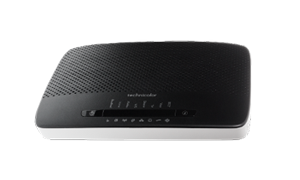
\includegraphics[width=0.5\textwidth]{images/tg799.png}
\caption{The TG799 router from Technicolor}
\label{fig:tg799}
\end{figure}

\section{IEEE 802.11}

As mentioned in the introduction, the IEEE 802.11 standard defines the
\emph{distributed coordination function} (DCF). This section aims to give the
reader enough understanding of the DCF to follow along in the arguments and
discussions. The reader is refered to the original 802.11 standard for a
complete definition \cite{654749}.



\section{ubus - the OpenWrt micro bus architecture}

A client program which acts as an interface to the bus daemon, \texttt{ubusd}.
Input and output format is JSON.

\section{Deutche telekom supra}

Björns oklara vapen.

\section{Rhode \& Schwarz FWLZ-XYZ}

(not broken) network analyser;

\section{Wi-Spy Channalyzer}

the wi-spy, top secret agent auf d00m.

\section{Wireshark, tshark}

Wireshark is a well-known program for capturing and inspecting network data
based around \texttt{libpcap}.

\section{jana}

A program, developed by the author of this thesis, for running network tests.
Supports expontential, uniform and gamma distributed packet send rate and
payload size. It is designed to be used together with packet capture software
(e.g. Wireshark) which enables a user to estimate the time from a `sendmsg`
syscall to the packet actually leaving the NIC. These features were developed
to facilitate experimental, yet controlled, evaluation of the theoretical IEEE
802.11 performance models.

\section{Linux Networking}

A high level view of a packet's way from the userspace program, through the
kernel and finally to the network interface responsible for physically
transmitting it can be found in \ref{fig:linux_egress}.

\begin{figure}
\center
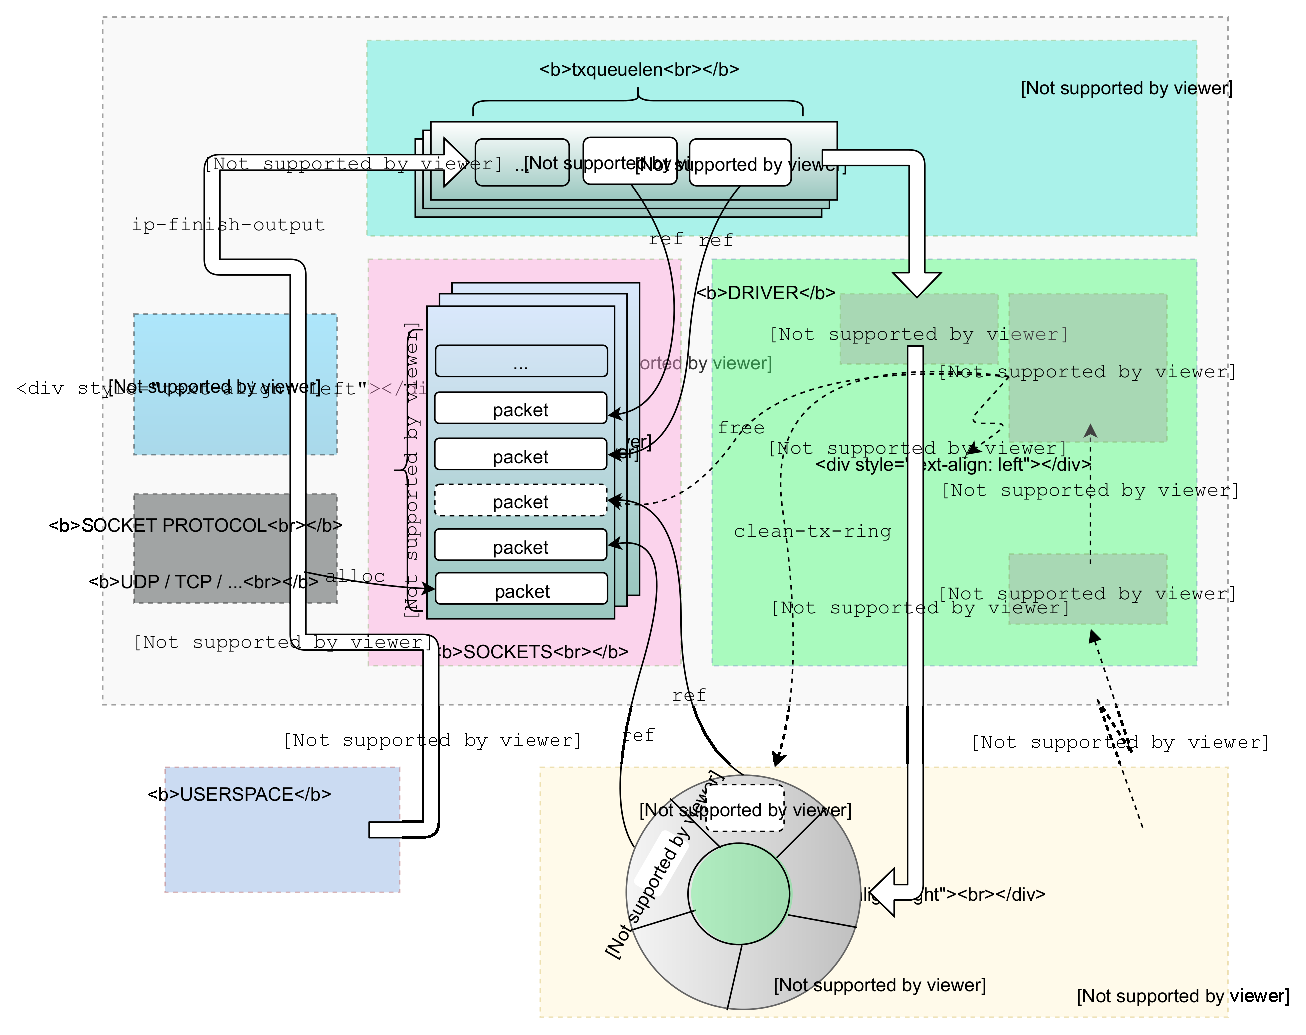
\includegraphics[width=0.9\textwidth]{images/linux-egress-overview.eps}
\caption{TG799 router and measurement antenna side by side, 1 meter from laptop}
\label{fig:linux_egress}
\end{figure}
